\documentclass{article}
\usepackage{tikz}
\usepackage{tikz-qtree}
\usepackage{forest}




\author{Lin Jiaying}
\title{Chap.5 Exercise}


\begin{document}
	
	\maketitle
	\section{Question 5.1 Answer: }
	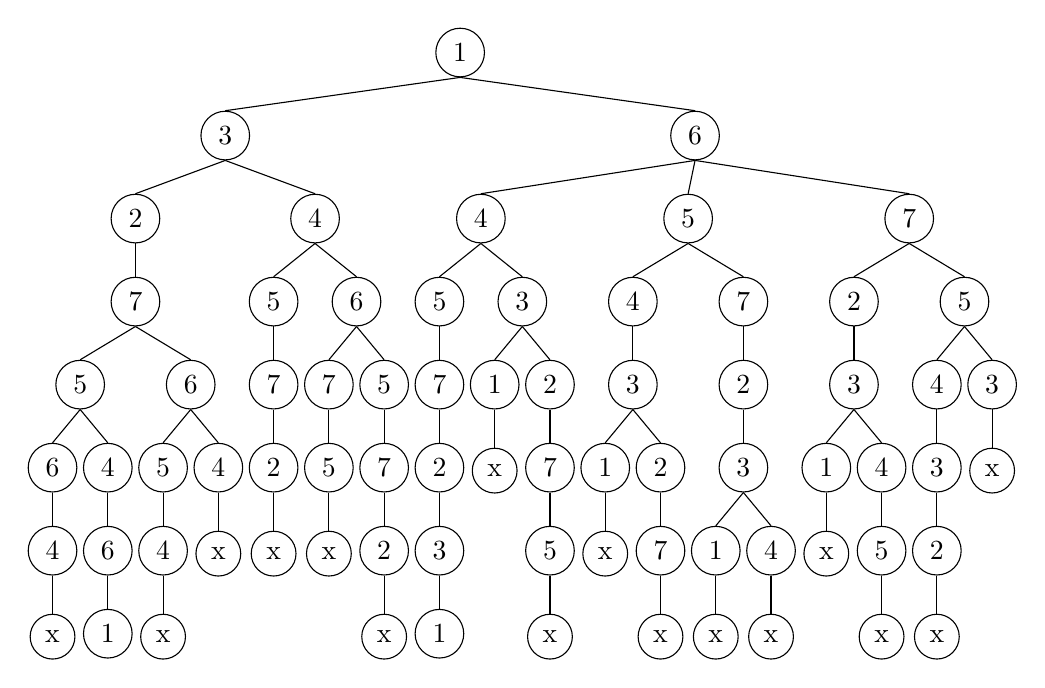
\begin{tikzpicture}[every internal node/.style={draw,circle}]
		\Tree
		[.1
	     [.3
	      [.2
	       [.7
	        [.5
	         [.6
	          [.4
	           [.x ]]]
	         [.4
	          [.6
	           [.1 ]]]]
	        [.6
	         [.5
	          [.4
	           [.x ]]]
	         [.4 [.x ]]]]]
	       [.4
	        [.5
	         [.7
	          [.2
	           [.x ]]]]
	        [.6
	         [.7
	          [.5
	           [.x ]] ]
	         [.5
	          [.7
	           [.2
	            [.x ]]] ]] ]]
	         [.6
	          [.4
	           [.5
	            [.7
	             [.2
	              [.3
	               [.1 ]]]]]
	           [.3 [.1 [.x ]]
	            [.2
	             [.7
	              [.5
	               [.x ]]]
	            ]]]
	          [.5
	            [.4 
	             [.3
	              [.1
	               [.x ]]
	              [.2
	               [.7
	                [.x ]]]]]
	             [.7
	              [.2
	               [.3 [.1 [.x ]]
	                [.4 
	                 [.x ]]]]]
	                ]
	           [.7
	           [.2 [.3 [.1 [.x ]] [.4 [.5 [.x ]]]]]
	            [.5
	             [.4 [.3 [.2 [.x ]]]]
	              [.3
	               [.x ]]]]]]
	          
	\end{tikzpicture}
	
	\section{Question 5.3 Answer:}
	\begin{forest}
	for tree={circle,draw, l sep=20pt}
	[$v_0$(0) 
		[$v_1$(1), edge label = {node[midway, left]{1}}		  
		  [$v_5$(4), edge label = {node[midway, left]{3}}
		   [$v_8$(6), edge label = {node[midway, left]{2}}]]
		[$v_6$(11), edge label = {node[midway, left]{10}} [$7>6$]]]
		[$v_2$(5), edge label = {node[midway, left]{5}}
		 [$v_5$(7), edge label = {node[midway, left]{2}} [$7>6$]]
		 [$v_7$(7), edge label = {node[midway, left]{2}} [$7>6$]]

	]
	[$v_3$(7), edge label = {node[midway, right]{7}} [$7>6$]]
	[$v_4$(4), edge label = {node[midway, right]{4}}
	 [$v_7$(7), edge label = {node[midway, right]{3}} [$7>6$]]]
	];
	\end{forest}
.\\
	So the shortest path we found is $v_0 \rightarrow v_1 \rightarrow v_5 \rightarrow v_8$(1 + 3 + 2 = 6).\\
	
	\section{Question 5.4 Answer:}
	The lower bound = 5 + 7 + 8 + 6 + 10 = 36.\\
	\begin{forest}
		for tree={draw, l sep=20pt}
		[All Solution\\
		Lower Bound:36, align=center, base=bottom
		 [All solution with 5-3\\
		 Lower Bound:36, align=center, base=bottom
		   [All solution with 3-4\\
		   Lower Bound:36, align=center, base=bottom
		    [All solution with 4-1\\
		    Lower Bound:36, align=center, base=bottom
		    [All solution with 2-5\\
		     Lower Bound:36, align=center, base=bottom
		    [All solution with 1-2\\
		    Lower Bound:36, align=center, base=bottom]
		    [All solution without 1-2\\
		    No solution, align=center, base=bottom]]
		    [All solution without 2-5\\
		    Lower Bound:43, align=center, base=bottom]]
		    [All solution without 4-1\\
		    Lower Bound:130, align=center, base=bottom]]
		    [All solution without 3-4\\
		    Lower Bound:80, align=center, base=bottom]]
		 [All solution without 5-3\\
		 Lower Bound:88, align=center, base=bottom]
		]
	\end{forest}
	Solution: $5\to3\to4\to1\to2\to5$.
\end{document}